
\section{Conclusion}

In this paper, we propose a new fine-tuning method for skill discovery for combining learned skills efficiently.
By combining skills on the representation level rather than an action level,
it is possible to generalize the previous method and outperform other unsupervised RL methods in a sample efficiency manner.
We emphasize the importance of fine-tuning method for measuring the performance for a skill discovery method
and encourage the research direction for other skill mix method for future work.


% In this paper, we propose a method to enable faster and better learning by combining the skills learned in the pretrain phase.
% The interesting thing is that it is better to have a skill weight regardless of the state than to have a different skill weight for each state.
% Based on these results, we want to find a way to better utilize skill combinations such as attention in the future.



% \subsection{Attention}
% \begin{figure}[hb]
%   \vskip 0.2in
%   \begin{center}
%   \centerline{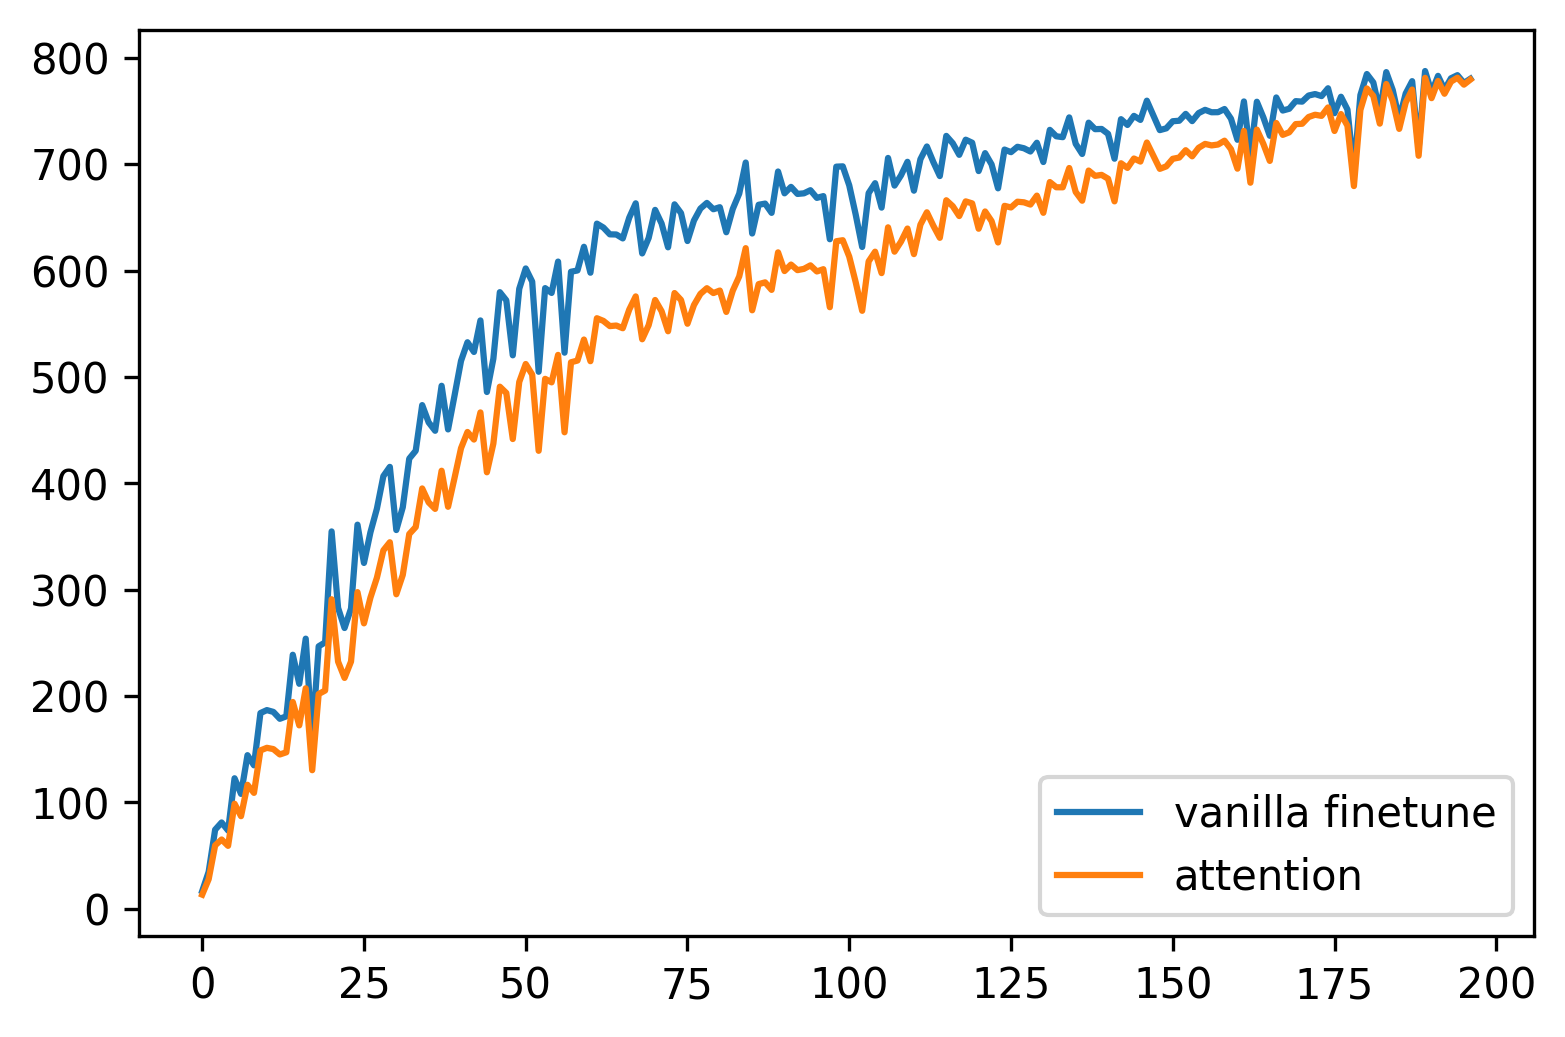
\includegraphics[width=\columnwidth]{Figures/attention_on_walker_run.png}}
%   \caption{This result was lost}
%   \label{attention-on-walker-run}
%   \end{center}
%   \vskip -0.2in
%   \end{figure}